The injection kicker magnets in the LHC are part of the injection system for the LHC machine. This system is used to match the trajectory of the injected beam to that of the stable beam path in the accelerator. An example schema for the LHC can be seen in Fig.~\ref{fig:injection-system-schema}. The system typically uses two components, a septum, which may provide a slowly rising and falling time, but strong, field, and kickers, which may provide a rapidly rising and falling, but comparatively weak field, to match the injected beam to the correct trajectory. Similar components are used for the extraction of beam also.

\begin{figure}
\begin{center}
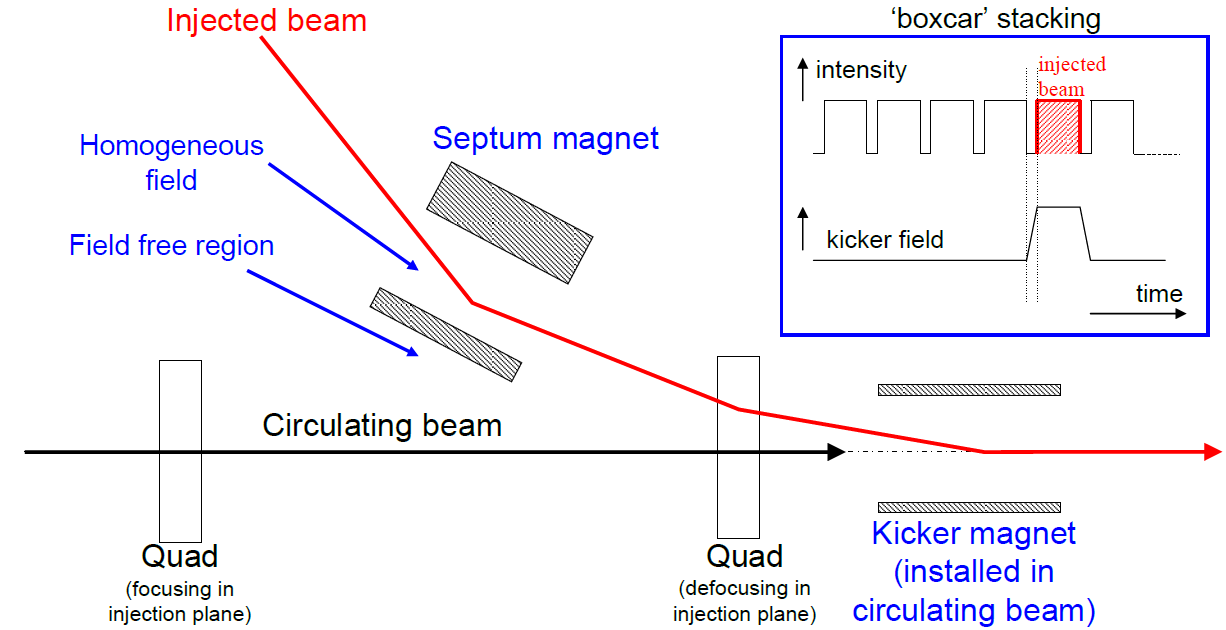
\includegraphics[width=0.6\textwidth]{LHC_MKI/figures/injection-system.png}
\end{center}
\caption{An example layout of a injection system for an accelerator. Taken from \cite{Barnes:injSys}}
\label{fig:injection-system-schema}
\end{figure}

By design kickers must always be visible to the beam due to the need to quickly fire to apply their kick. In addition the need for a highly homogeneous field whilst the kick is applied, as well as the strength of the field neccesitates that the aperture for kickers often be very narrow, meaning they are in close proximity to the beam. This leads to two concerns - that the close proximity of the beam to a device that may be made of either a highly lossy material \cite{Day:wireMeasFerr, Barnes:wireMeasKick, Barnes:spsKickerHeating} or of a source of strong geometrical impedance \cite{Belver-Aguilar:clicStripline} may be source of impedance that drives instabilities in the beam [impedance of the SPS], and secondly that the large real component of ferrite kicker magnets may be subject to intense heating in high beam current machines \cite{Barnes:spsKickerHeating}. 

\section{LHC Injection Kicker Magnets}

The LHC injection kicker magnets (LHC-MKIs, or MKI) are a 3m long travelling wave transmission line kicker magnet (ferrite length 2.7m). For LHC there are two injection regions, at near IPs 2 and 8, each consisting of an septa system and four MKIs injecting vertically into the machine (The position of the LHC injection systems is shown in Fig.~\ref{fig:lhc-injection-systems}). As a transmission line magnet the magnet is constructed of a c-core ferrite yoke, segmented by alternating HV and ground plates capacitively coupled together by ceramic capacitor plates. The pulse is generator in a pulse forming network (PFN), stationed above ground, which is subsequently carried by a cable with a characteristic impedance of $5 \Omega$, matching the characteristic impedance of the MKI. The performance parameters of the magnets rise time, fied strength and homogeneity are given in Tab.~\ref{tab:mki-parameters} \cite{Ducimetière:mkiSpec}.

\begin{figure}
\begin{center}
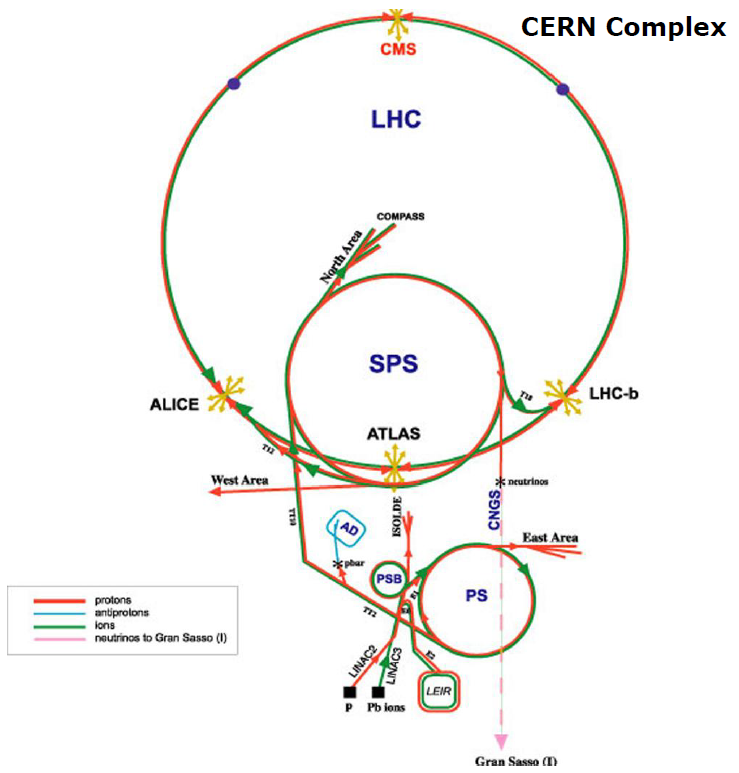
\includegraphics[width=0.6\textwidth]{LHC_MKI/figures/injection-points-lhc.png}
\end{center}
\label{fig:lhc-injection-systems}
\caption{The location of the LHC injection systems in the LHC ring.}
\end{figure}


\begin{figure}
\begin{center}
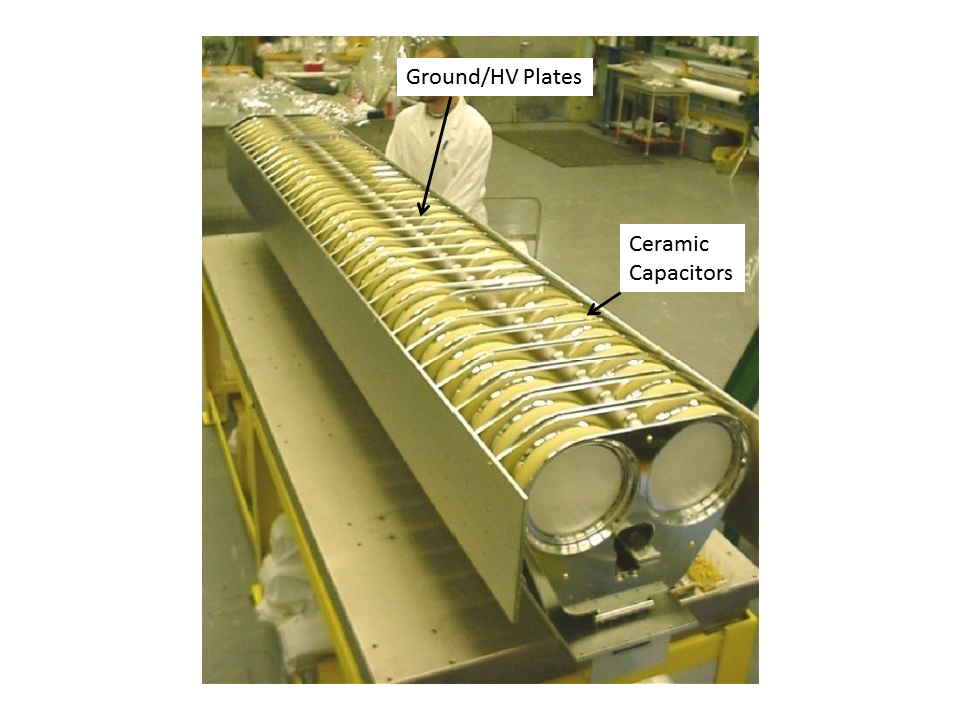
\includegraphics[height=0.4\textwidth]{LHC_MKI/figures/mki-out-vac-tank.png}
\end{center}
\label{fig:lhc-mki-cross-section}
\caption{\ref{fig:lhc-mki-cross-section} A cross section of an MKI. Visible are the alternating HV and ground plates, seperated by capacitor plates. The HV drive plate and the ground return can be seen in the c core of the ferrite yoke.}
\end{figure}

\begin{table}
\caption{MKI Operational parameters}

\begin{center}
\begin{tabular}{c | c | c}
Number of Kickers per System & 4 & \\ \hline
Kick strength per magnet & 0.3 & T.m \\ \hline
Magnet beam aperture (diameter) & 38 & mm \\ \hline
Characteristic Impedance & 5 & $\Omega$ \\ \hline
Operating charging voltage (PFN) & 54 & kV \\ \hline
Field flat top ripple & < $\pm$0.5 & \% \\ \hline
Field flat top duration & up to 7.86 & $\mu$ s \\ \hline
Field rise time 0.5\%-99.5\% & 0.9 & $\mu$ s \\ \hline
Field fall time 99.5\%-0.5\% & 3.0 & $\mu$ s \\ \hline
Magnet kength & 2.7 & m \\ 
\end{tabular}
\end{center}
\label{tab:mki-parameters}
\end{table}